\documentclass[10pt,a4paper]{article}

\usepackage[utf8]{inputenc}
\usepackage[T1]{fontenc}
\usepackage[english]{babel}
\usepackage{lmodern}
\usepackage{microtype}
\usepackage[a4paper,top=1.7cm,bottom=1.8cm,left=1.55cm,right=1.55cm,headheight=13pt]{geometry}
\usepackage{amsmath,amssymb,mathtools,bm}
\mathtoolsset{showonlyrefs}
\usepackage{booktabs,tabularx,array}
\usepackage{xcolor}
\usepackage{tikz}
\usetikzlibrary{babel}
\usepackage{float}
\usepackage{fancyhdr}
\usepackage{enumitem}
\usepackage[hidelinks]{hyperref}
\usepackage[most]{tcolorbox}

\definecolor{navy}{HTML}{17365D}
\definecolor{teal}{HTML}{167D7F}
\definecolor{gold}{HTML}{C78B24}
\definecolor{softblue}{HTML}{EEF4F8}
\definecolor{softgold}{HTML}{FFF7E8}
\definecolor{softgray}{HTML}{F3F4F6}
\definecolor{darkgray}{HTML}{374151}

\hypersetup{
  pdftitle={Commutation Condition and Order Invariance in Bimaterial Dielectric Stacks under TM Polarization},
  pdfauthor={Nahuel Alejandro Roldan},
  pdfsubject={Commutation of transfer matrices in bimaterial dielectric thin films}
}

\pagestyle{fancy}
\fancyhf{}
\lhead{\textcolor{navy}{\small TMM and commutativity in thin films}}
\rhead{\textcolor{darkgray}{\small Derivation}}
\cfoot{\textcolor{darkgray}{\thepage}}
\renewcommand{\headrulewidth}{0.4pt}

\setlength{\parindent}{0pt}
\setlength{\parskip}{3pt}
\setlength{\columnsep}{0.68cm}
\renewcommand{\dbltopfraction}{0.95}
\renewcommand{\dblfloatpagefraction}{0.80}
\setcounter{dbltopnumber}{2}
\setlength{\abovedisplayskip}{5pt plus 2pt minus 2pt}
\setlength{\belowdisplayskip}{5pt plus 2pt minus 2pt}
\setlist[itemize]{leftmargin=1.3em,itemsep=1pt,topsep=2pt}
\setlist[enumerate]{leftmargin=1.7em,itemsep=1pt,topsep=2pt}

\newcommand{\ii}{\mathrm{i}}
\newcommand{\M}{\mathbf{M}}
\newcommand{\B}{\mathbf{B}}
\newcommand{\I}{\mathbf{I}}
\newcommand{\comm}[2]{\left[#1,#2\right]}
\newcommand{\qab}{q_{\mathrm{ab}}}
\newcommand{\vE}{\vec{E}}
\newcommand{\vH}{\vec{H}}
\newcommand{\vk}{\vec{k}}
\newcommand{\vPsi}{\vec{\Psi}}

\newtcolorbox{resultbox}{
  colback=softblue,
  colframe=navy,
  boxrule=0.8pt,
  arc=1.5mm,
  left=3mm,right=3mm,top=2mm,bottom=2mm
}
\newtcolorbox{warningbox}{
  colback=softgold,
  colframe=gold,
  boxrule=0.8pt,
  arc=1.5mm,
  left=3mm,right=3mm,top=2mm,bottom=2mm
}

\begin{document}

\twocolumn[
\begin{center}
  {\Large\bfseries\color{navy}
  Commutation Condition and Order Invariance in Bimaterial
  Dielectric Stacks under TM Polarization}\par
  \vspace{4pt}
  {\normalsize Derivation using transfer matrices and commutators}\par
  \vspace{4pt}
  {\small\bfseries Nahuel Alejandro Rold\'an}\par
  {\footnotesize National Scientific and Technical Research Council (CONICET)}\par
  {\footnotesize
  ORCID: \href{https://orcid.org/0009-0009-6747-0756}{0009-0009-6747-0756}
  \quad Version 0.1 \quad October 7, 2026 \quad CC BY 4.0}\par
  {\footnotesize Preprint, not peer reviewed}
\end{center}

\begin{minipage}{0.92\textwidth}
\small
\textbf{Abstract.} We derive a sufficient condition under which the characteristic matrices of two dielectric materials $H$ and $L$ commute independently of their thicknesses. Starting from Maxwell's equations, we construct the transfer matrix of a single layer and explicitly evaluate the vanishing of its commutator. For TM polarization, the resulting incidence angle is
\begin{equation}
\boxed{
\theta_{\mathrm{ab}}
=
\arcsin\!\left(
\frac{n_Hn_L}{n_0\sqrt{n_H^2+n_L^2}}
\right)}.
\label{eq:resultado-principal}
\end{equation}
Under this condition, the total product depends on accumulated phases and loses its dependence on layer order. We also state the assumptions under which this reduction is exact.

\medskip
\textbf{Keywords.} Thin films; transfer-matrix method; matrix commutation; order invariance; TM polarization.
\end{minipage}
\vspace{7pt}
]

\section{Maxwell equations and stratified media}

We consider linear, homogeneous, isotropic media without free sources, with harmonic time dependence $e^{-\ii\omega t}$. The macroscopic Maxwell equations are~[1]
\begin{align}
\vec{\nabla}\cdot\vE&=0,
&\vec{\nabla}\cdot\vH&=0,\\
\vec{\nabla}\times\vE&=\frac{\ii\omega\mu}{c}\vH,
&\vec{\nabla}\times\vH&=-\frac{\ii\omega\varepsilon}{c}\vE,
\label{eq:maxwell}
\end{align}
with constitutive relations
\begin{equation}
\vec D=\varepsilon\vE,
\qquad
\vec B=\mu\vH.
\label{eq:constitutivas}
\end{equation}
The structure is stratified along $\hat y$ and is invariant within the plane of each interface. We choose the $x$--$y$ plane of incidence and write
\begin{equation}
\vk=\alpha\hat x+\beta\hat y.
\label{eq:k-vector}
\end{equation}
The tangential component $\alpha$ must be the same in every medium. If the beam is incident from a medium with refractive index $n_0$ at angle $\theta_0$,
\begin{equation}
\alpha=k_0n_0\sin\theta_0,
\qquad
k_0=\frac{\omega}{c}=\frac{2\pi}{\lambda}.
\label{eq:alpha}
\end{equation}
In layer $j$, the dispersion relation $|\vk_j|^2=k_0^2\varepsilon_j\mu_j=k_0^2n_j^2$ gives
\begin{align}
\beta_j^{\pm}
&=\pm\sqrt{k_0^2n_j^2-\alpha^2}\\
&=\pm k_0\sqrt{n_j^2-n_0^2\sin^2\theta_0}
=\pm k_0n_j\cos\theta_j.
\label{eq:beta}
\end{align}
This identity contains Snell's law,
\begin{equation}
n_0\sin\theta_0=n_j\sin\theta_j.
\label{eq:snell}
\end{equation}

\begin{figure*}[t]
\centering
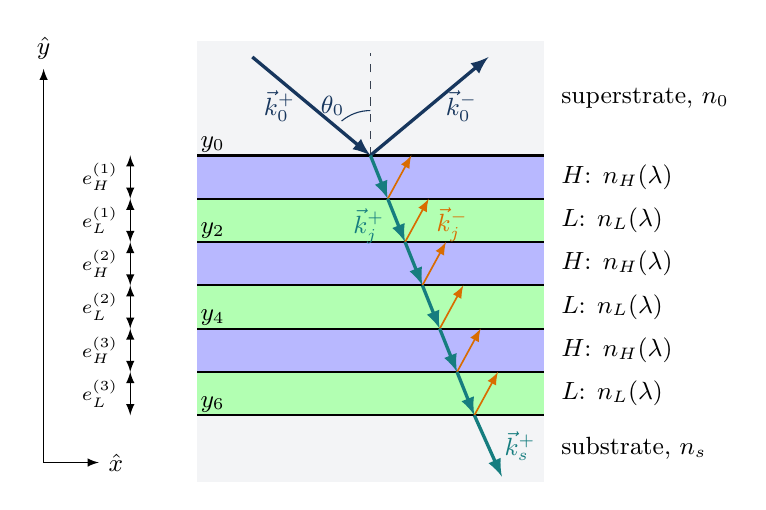
\begin{tikzpicture}[x=1cm,y=1cm,>=latex,font=\small]
  \fill[softgray] (-2.2,3.60) rectangle (2.2,5.05);
  \fill[blue!28]  (-2.2,3.05) rectangle (2.2,3.60);
  \fill[green!30] (-2.2,2.50) rectangle (2.2,3.05);
  \fill[blue!28]  (-2.2,1.95) rectangle (2.2,2.50);
  \fill[green!30] (-2.2,1.40) rectangle (2.2,1.95);
  \fill[blue!28]  (-2.2,0.85) rectangle (2.2,1.40);
  \fill[green!30] (-2.2,0.30) rectangle (2.2,0.85);
  \fill[softgray] (-2.2,-0.55) rectangle (2.2,0.30);
  \foreach \y in {3.60,3.05,2.50,1.95,1.40,0.85,0.30}
    \draw[thick] (-2.2,\y)--(2.2,\y);
  \draw[dashed,darkgray] (0,3.60)--(0,4.90);
  \draw[very thick,navy,->] (-1.50,4.85)--(0,3.60)
    node[midway,left=2pt] {$\vk_0^{+}$};
  \draw[very thick,navy,->] (0,3.60)--(1.50,4.85)
    node[midway,right=2pt] {$\vk_0^{-}$};

  % The forward and reflected branches are shown simultaneously in each layer.
  \draw[very thick,teal,->] (0.00,3.60)--(0.22,3.05);
  \draw[semithick,orange!85!black,->] (0.22,3.05)--(0.52,3.60);
  \draw[very thick,teal,->] (0.22,3.05)--(0.44,2.50);
  \draw[semithick,orange!85!black,->] (0.44,2.50)--(0.74,3.05);
  \draw[very thick,teal,->] (0.44,2.50)--(0.66,1.95);
  \draw[semithick,orange!85!black,->] (0.66,1.95)--(0.96,2.50);
  \draw[very thick,teal,->] (0.66,1.95)--(0.88,1.40);
  \draw[semithick,orange!85!black,->] (0.88,1.40)--(1.18,1.95);
  \draw[very thick,teal,->] (0.88,1.40)--(1.10,0.85);
  \draw[semithick,orange!85!black,->] (1.10,0.85)--(1.40,1.40);
  \draw[very thick,teal,->] (1.10,0.85)--(1.32,0.30);
  \draw[semithick,orange!85!black,->] (1.32,0.30)--(1.62,0.85);
  \draw[very thick,teal,->] (1.32,0.30)--(1.67,-0.48)
    node[midway,right=2pt] {$\vk_s^{+}$};
  \node[teal] at (-0.02,2.70) {$\vk_j^{+}$};
  \node[orange!85!black] at (1.04,2.72) {$\vk_j^{-}$};

  \draw[navy] (0,4.17) arc[start angle=90,end angle=130,radius=0.57];
  \node[navy] at (-0.48,4.23) {$\theta_0$};
  \draw[->] (-4.15,-0.30)--(-4.15,4.70) node[above] {$\hat y$};
  \draw[->] (-4.15,-0.30)--(-3.45,-0.30) node[right] {$\hat x$};

  \foreach \ya/\yb/\lab in {
    3.05/3.60/$e_H^{(1)}$,2.50/3.05/$e_L^{(1)}$,
    1.95/2.50/$e_H^{(2)}$,1.40/1.95/$e_L^{(2)}$,
    0.85/1.40/$e_H^{(3)}$,0.30/0.85/$e_L^{(3)}$}
    {\draw[<->] (-3.05,\ya)--(-3.05,\yb);
     \node[left,font=\scriptsize] at (-3.08,{(\ya+\yb)/2}) {\lab};}

  \node[right] at (2.30,4.32) {superstrate, $n_0$};
  \node[right] at (2.30,3.325) {$H$: $n_H(\lambda)$};
  \node[right] at (2.30,2.775) {$L$: $n_L(\lambda)$};
  \node[right] at (2.30,2.225) {$H$: $n_H(\lambda)$};
  \node[right] at (2.30,1.675) {$L$: $n_L(\lambda)$};
  \node[right] at (2.30,1.125) {$H$: $n_H(\lambda)$};
  \node[right] at (2.30,0.575) {$L$: $n_L(\lambda)$};
  \node[right] at (2.30,-0.12) {substrate, $n_s$};
  \node[above right,inner sep=1pt] at (-2.2,3.60) {$y_0$};
  \node[above right,inner sep=1pt] at (-2.2,2.50) {$y_2$};
  \node[above right,inner sep=1pt] at (-2.2,1.40) {$y_4$};
  \node[above right,inner sep=1pt] at (-2.2,0.30) {$y_6$};
\end{tikzpicture}
\caption{One-dimensional bimaterial structure with six horizontal layers. Green arrows denote transmitted components and orange arrows denote reflected components generated at each interface. The branching illustrates the coexistence of forward- and backward-propagating waves in every layer; outside the Abelian limit, the microscopic $H/L$ sequence is encoded in the ordered matrix product.}
\label{fig:stack-hl}
\end{figure*}

The two polarizations decouple. For TE, $\vE_j$ is parallel to $\hat z$; for TM, $\vH_j$ is parallel to $\hat z$. We define the scalar field
\begin{equation}
f_j(x,y)=
\begin{cases}
E_{z,j}(x,y),&\mathrm{TE},\\
H_{z,j}(x,y),&\mathrm{TM},
\end{cases}
\end{equation}
and the parameter accompanying its normal derivative,
\begin{equation}
\sigma_j=
\begin{cases}
\mu_j,&\mathrm{TE},\\
\varepsilon_j,&\mathrm{TM}.
\end{cases}
\label{eq:sigma}
\end{equation}
The solution within a layer is the superposition of the two branches of $\beta_j$:
\begin{equation}
f_j(x,y)=
\left(A_j e^{-\ii\beta_j y}+B_j e^{\ii\beta_j y}\right)e^{\ii\alpha x}.
\label{eq:onda-capa}
\end{equation}
Here $A_j$ and $B_j$ are the forward and backward amplitudes, respectively.

\section{Boundary conditions and TMM}

At an interface $y=y_j$ there are no surface currents or charges. Continuity of the tangential components of $\vE$ and $\vH$ is equivalent to
\begin{align}
f_j(x,y_j)&=f_{j+1}(x,y_j),\\
\frac{1}{\sigma_j}\frac{\partial f_j}{\partial y}(x,y_j)
&=\frac{1}{\sigma_{j+1}}\frac{\partial f_{j+1}}{\partial y}(x,y_j).
\label{eq:borde}
\end{align}
Substituting Eq.~\eqref{eq:onda-capa} and cancelling the common factor $e^{\ii\alpha x}$ gives
\begin{equation}
\underbrace{\begin{pmatrix}
e^{-\ii\beta_j y_j}&e^{\ii\beta_j y_j}\\[2pt]
-\dfrac{\beta_j}{\sigma_j}e^{-\ii\beta_j y_j}&
\dfrac{\beta_j}{\sigma_j}e^{\ii\beta_j y_j}
\end{pmatrix}}_{\mathbf{G}_j(y_j)}
\begin{pmatrix}A_j\\B_j\end{pmatrix}
=
\mathbf{G}_{j+1}(y_j)
\begin{pmatrix}A_{j+1}\\B_{j+1}\end{pmatrix}.
\label{eq:interfaz-matricial}
\end{equation}
Therefore, amplitude transfer across an interface is
\begin{equation}
\begin{pmatrix}A_j\\B_j\end{pmatrix}
=\mathbf{G}_j(y_j)^{-1}\mathbf{G}_{j+1}(y_j)
\begin{pmatrix}A_{j+1}\\B_{j+1}\end{pmatrix}.
\label{eq:transferencia-interfaz}
\end{equation}
Chaining all interfaces produces the ordered product relating the superstrate and substrate. If no wave is incident from the substrate, $B_s=0$, and
\begin{equation}
R=\left|\frac{B_0}{A_0}\right|^2.
\label{eq:R-amplitudes}
\end{equation}

To study the contribution of each layer, it is convenient to replace the amplitudes $(A_j,B_j)$ with a tangential-field state vector
\begin{equation}
\vPsi_j(y)=
\begin{pmatrix}
f_j(y)\\[2pt]
g_j(y)
\end{pmatrix},
\qquad
g_j(y)\propto\frac{1}{\sigma_j}\frac{\partial f_j}{\partial y}.
\label{eq:vector-estado}
\end{equation}
Both entries are continuous across every interface. Propagating this state between the two faces of layer $j$ yields the characteristic matrix
\begin{equation}
\vPsi_j(y_j)=\M_j\,\vPsi_j(y_j+e_j),
\end{equation}
\begin{equation}
\M_j(\varphi_j,q_j)=
\begin{pmatrix}
\cos\varphi_j & \ii q_j^{-1}\sin\varphi_j\\[2pt]
\ii q_j\sin\varphi_j & \cos\varphi_j
\end{pmatrix},
\label{eq:matriz-capa}
\end{equation}
where
\begin{equation}
\varphi_j=\beta_j e_j
=\frac{2\pi}{\lambda}n_je_j\cos\theta_j
\label{eq:fase}
\end{equation}
and, with the normalization adopted here,
\begin{align}
q_j^{\mathrm{TE}}&=n_j\cos\theta_j,
\label{eq:qte}\\
q_j^{\mathrm{TM}}&=\frac{\cos\theta_j}{n_j}.
\label{eq:qtm}
\end{align}
Using the reciprocal TM admittance exchanges $q_j$ with $q_j^{-1}$ but does not change the equality condition between materials. For $N$ layers,
\begin{align}
\M_{\mathrm{tot}}
&=\M_1\M_2\cdots\M_N,
\label{eq:producto-total}
\end{align}
with explicit factors
\begin{align*}
\M_1&=
\begin{pmatrix}
\cos\varphi_1 & \ii q_1^{-1}\sin\varphi_1\\
\ii q_1\sin\varphi_1 & \cos\varphi_1
\end{pmatrix},\\[2pt]
\M_2&=
\begin{pmatrix}
\cos\varphi_2 & \ii q_2^{-1}\sin\varphi_2\\
\ii q_2\sin\varphi_2 & \cos\varphi_2
\end{pmatrix},\\[-2pt]
&\hspace{1.2cm}\vdots\\[-2pt]
\M_N&=
\begin{pmatrix}
\cos\varphi_N & \ii q_N^{-1}\sin\varphi_N\\
\ii q_N\sin\varphi_N & \cos\varphi_N
\end{pmatrix}.
\end{align*}
Each factor contains the phase $\varphi_j=\beta_j e_j$ and the reduced admittance
$q_j$ of its own layer. This ordering is not merely notational: in general,
$\M_i\M_j\neq\M_j\M_i$. Hence, exchanging two factors changes
$\M_{\mathrm{tot}}$ and therefore the reflectance.

\section{Idea: converting the product into a sum}

The algebraic motivation is to compress the product in Eq.~\eqref{eq:producto-total}. If every invertible matrix locally admits a logarithm, we may introduce a generator $\mathbf{A}_j$ such that
\begin{equation}
\M_j=e^{\mathbf{A}_j},
\qquad
\mathbf{A}_j=\log\M_j.
\label{eq:log-general}
\end{equation}
We would like to replace
\begin{equation}
e^{\mathbf{A}_1}e^{\mathbf{A}_2}\cdots e^{\mathbf{A}_N}
\quad\hbox{by}\quad
e^{\mathbf{A}_1+\mathbf{A}_2+\cdots+\mathbf{A}_N}.
\label{eq:deseo-aditivo}
\end{equation}
This is the matrix analogue of the elementary product rule for scalar exponentials, but it does not hold for arbitrary matrices. The Campbell--Baker--Hausdorff formula shows that
\begin{equation}
\log\!\left(e^{\mathbf{A}_1}e^{\mathbf{A}_2}\right)
=\mathbf{A}_1+\mathbf{A}_2+\frac{1}{2}\comm{\mathbf{A}_1}{\mathbf{A}_2}+\cdots.
\label{eq:bch-motivacion}
\end{equation}
Consequently, exact additive reduction occurs when the generators commute. The physical question becomes: \emph{can the conditions $C$---in particular $\theta_0$ and the polarization---be chosen so that the matrices of $H$ and $L$ commute for arbitrary thicknesses?}

We do not answer this question by postulating an abstract generator. Instead, we derive it from the layer matrix itself.

We define
\begin{equation}
\B(q)=
\begin{pmatrix}
0&q^{-1}\\
q&0
\end{pmatrix}.
\label{eq:Bq}
\end{equation}
Direct multiplication of the generator in Eq.~\eqref{eq:Bq} gives
\begin{equation}
\B(q)^2=\I.
\label{eq:B2}
\end{equation}
Therefore, the exponential series separates into even and odd powers:
\begin{align}
\exp\!\left(\ii\varphi\B\right)
&=\sum_{m=0}^{\infty}\frac{(\ii\varphi\B)^m}{m!}\\
&=\I\sum_{r=0}^{\infty}\frac{(-1)^r\varphi^{2r}}{(2r)!}
+\ii\B\sum_{r=0}^{\infty}\frac{(-1)^r\varphi^{2r+1}}{(2r+1)!}\\
&=\I\cos\varphi+\ii\B\sin\varphi.
\end{align}
We now substitute explicitly the two matrices appearing in the last line:
\begin{align*}
\I\cos\varphi
&=\cos\varphi
\begin{pmatrix}
1&0\\0&1
\end{pmatrix}
\nonumber\\
&=
\begin{pmatrix}
\cos\varphi&0\\0&\cos\varphi
\end{pmatrix},
\\[4pt]
\ii\B(q)\sin\varphi
&=\ii\sin\varphi
\begin{pmatrix}
0&q^{-1}\\q&0
\end{pmatrix}
\nonumber\\
&=
\begin{pmatrix}
0&\ii q^{-1}\sin\varphi\\
\ii q\sin\varphi&0
\end{pmatrix}.
\end{align*}
Adding the entries componentwise,
\begin{align*}
\I\cos\varphi+\ii\B(q)\sin\varphi
&=
\begin{pmatrix}
\cos\varphi+0&0+\ii q^{-1}\sin\varphi\\
0+\ii q\sin\varphi&\cos\varphi+0
\end{pmatrix}
\\[3pt]
&=
\begin{pmatrix}
\cos\varphi&\ii q^{-1}\sin\varphi\\
\ii q\sin\varphi&\cos\varphi
\end{pmatrix}.
\end{align*}
This matrix agrees entry by entry with the characteristic matrix in Eq.~\eqref{eq:matriz-capa}. Therefore,
\begin{equation}
\boxed{\M_j=\exp\!\left(\ii\varphi_j\B(q_j)\right).}
\label{eq:exponencial}
\end{equation}
The exponential representation~\eqref{eq:exponencial} makes the algebraic generator of each layer explicit.

\section{Commutator of two layers}

Consider two layers $i$ and $j$. We first compute the products of their generators:
\begin{align}
\B(q_i)\B(q_j)
&=
\begin{pmatrix}
q_j/q_i&0\\
0&q_i/q_j
\end{pmatrix},\\[3pt]
\B(q_j)\B(q_i)
&=
\begin{pmatrix}
q_i/q_j&0\\
0&q_j/q_i
\end{pmatrix}.
\end{align}
Hence,
\begin{equation}
\comm{\B(q_i)}{\B(q_j)}
=
\left(\frac{q_j}{q_i}-\frac{q_i}{q_j}\right)
\begin{pmatrix}1&0\\0&-1\end{pmatrix}.
\label{eq:conmutador-B}
\end{equation}
Since
\begin{equation}
\frac{q_j}{q_i}-\frac{q_i}{q_j}
=\frac{q_j^2-q_i^2}{q_iq_j},
\end{equation}
we obtain
\begin{equation}
\comm{\B(q_i)}{\B(q_j)}=0
\quad\Longleftrightarrow\quad
q_i^2=q_j^2.
\label{eq:condicion-q}
\end{equation}

Here $q_i$ and $q_j$ are the reduced layer admittances and depend on polarization. For $\ell\in\{i,j\}$,
\begin{equation*}
q_\ell=
\begin{cases}
q_\ell^{\mathrm{TE}}=n_\ell\cos\theta_\ell,
&\mathrm{TE},\\[2pt]
q_\ell^{\mathrm{TM}}=\dfrac{\cos\theta_\ell}{n_\ell},
&\mathrm{TM}.
\end{cases}
\end{equation*}
Therefore, the condition in Eq.~\eqref{eq:condicion-q} explicitly means
\begin{equation*}
\begin{aligned}
n_i^2\cos^2\theta_i&=n_j^2\cos^2\theta_j,
&&\mathrm{TE},\\
\frac{\cos^2\theta_i}{n_i^2}
&=\frac{\cos^2\theta_j}{n_j^2},
&&\mathrm{TM}.
\end{aligned}
\end{equation*}

The same condition follows directly for the layer matrices. To show this without omitting steps, write
\begin{equation*}
\M_\ell=c_\ell\I+\ii s_\ell\B_\ell,
\qquad
c_\ell=\cos\varphi_\ell,
\qquad
s_\ell=\sin\varphi_\ell.
\end{equation*}
The product in the order $i$ followed by $j$ is
\begin{align*}
\M_i\M_j
&=(c_i\I+\ii s_i\B_i)(c_j\I+\ii s_j\B_j)
\\
&=c_ic_j\I+\ii c_is_j\B_j+\ii s_ic_j\B_i-s_is_j\B_i\B_j.
\end{align*}
Reversing the order gives
\begin{align*}
\M_j\M_i
&=(c_j\I+\ii s_j\B_j)(c_i\I+\ii s_i\B_i)
\\
&=c_ic_j\I+\ii s_ic_j\B_i+\ii c_is_j\B_j-s_is_j\B_j\B_i.
\end{align*}
The terms proportional to $\I$, $\B_i$, and $\B_j$ are identical in both products and cancel upon subtraction. By definition,
\begin{align}
\comm{\M_i}{\M_j}
&=\M_i\M_j-\M_j\M_i
\nonumber\\
&=-s_is_j\left(\B_i\B_j-\B_j\B_i\right)
\nonumber\\
&=-\sin\varphi_i\sin\varphi_j\comm{\B_i}{\B_j}.
\label{eq:conmutador-M}
\end{align}
Identity~\eqref{eq:conmutador-M} separates the two effects: thickness dependence is contained in $\sin\varphi_i\sin\varphi_j$, whereas structural commutation is determined by $\comm{\B_i}{\B_j}$.

\begin{warningbox}
\textbf{Two types of commutation.}
\begin{itemize}
\item If $\sin\varphi_i=0$ or $\sin\varphi_j=0$, the commutator may vanish for particular thicknesses. This is an accidental, wavelength-dependent cancellation.
\item If $q_i^2=q_j^2$, the commutator vanishes for arbitrary phases and thicknesses. This is the structural commutation defining the Abelian limit.
\end{itemize}
\end{warningbox}

For passive media with positive admittances, the usual physical branch is $q_i=q_j$.

\section{TM solution}

We apply condition~\eqref{eq:condicion-q} to two materials $H$ and $L$. We first make all relevant quantities explicit. From Snell's law, Eq.~\eqref{eq:snell},
\begin{equation}
\sin\theta_j=\frac{n_0}{n_j}\sin\theta_0,
\end{equation}
and therefore
\begin{equation}
\cos^2\theta_j
=1-\frac{n_0^2}{n_j^2}\sin^2\theta_0
=\frac{n_j^2-n_0^2\sin^2\theta_0}{n_j^2}.
\label{eq:cos2}
\end{equation}
The normal component of the wave vector is
\begin{align}
\beta_j
&=k_0n_j\cos\theta_j
\nonumber\\
&=k_0\sqrt{n_j^2-n_0^2\sin^2\theta_0},
\qquad
k_0=\frac{2\pi}{\lambda}.
\label{eq:beta-seccion-tm}
\end{align}
Hence, the phase acquired in a layer of thickness $e_j$ is
\begin{align}
\varphi_j
&=\beta_j e_j
\nonumber\\
&=\frac{2\pi e_j}{\lambda}
\sqrt{n_j^2-n_0^2\sin^2\theta_0}.
\label{eq:phi-explicita-tm}
\end{align}
The thickness appears in $\varphi_j$ but not in the reduced admittance. For TM polarization, using Eq.~\eqref{eq:qtm} and $\beta_j=k_0n_j\cos\theta_j$,
\begin{align}
q_j^{\mathrm{TM}}
&=\frac{\cos\theta_j}{n_j}
\nonumber\\
&=\frac{\beta_j}{k_0n_j^2}
\nonumber\\
&=\frac{\sqrt{n_j^2-n_0^2\sin^2\theta_0}}{n_j^2}.
\label{eq:qtm-beta}
\end{align}
Squaring gives
\begin{equation}
\left(q_j^{\mathrm{TM}}\right)^2
=\frac{\cos^2\theta_j}{n_j^2}
=\frac{n_j^2-n_0^2\sin^2\theta_0}{n_j^4}.
\label{eq:qtm2}
\end{equation}
We impose equality between $H$ and $L$:
\begin{equation}
\frac{n_H^2-n_0^2\sin^2\theta_{\mathrm{ab}}}{n_H^4}
=
\frac{n_L^2-n_0^2\sin^2\theta_{\mathrm{ab}}}{n_L^4}.
\label{eq:igualdad-tm}
\end{equation}
For brevity, define
\begin{equation}
s=n_0^2\sin^2\theta_{\mathrm{ab}}.
\end{equation}
Multiplying Eq.~\eqref{eq:igualdad-tm} by $n_H^4n_L^4$ gives
\begin{align}
n_L^4(n_H^2-s)&=n_H^4(n_L^2-s),\\
s(n_H^4-n_L^4)&=n_H^4n_L^2-n_L^4n_H^2.
\end{align}
Factoring both sides,
\begin{align}
n_H^4-n_L^4&=(n_H^2-n_L^2)(n_H^2+n_L^2),\\
n_H^4n_L^2-n_L^4n_H^2&=n_H^2n_L^2(n_H^2-n_L^2).
\end{align}
If $n_H\neq n_L$, the factor $n_H^2-n_L^2$ cancels and yields
\begin{equation}
s=\frac{n_H^2n_L^2}{n_H^2+n_L^2}.
\end{equation}
Restoring the definition of $s$,
\begin{equation}
\boxed{
\sin^2\theta_{\mathrm{ab}}
=
\frac{n_H^2n_L^2}{n_0^2(n_H^2+n_L^2)}.}
\label{eq:sin2-ab}
\end{equation}
Taking the branch $0\leq\theta_{\mathrm{ab}}<\pi/2$, the quadratic relation~\eqref{eq:sin2-ab} leads to Eq.~\eqref{eq:resultado-principal}.

\subsection*{Existence condition}

The argument of the inverse sine must lie in $[0,1]$:
\begin{equation}
\frac{n_Hn_L}{n_0\sqrt{n_H^2+n_L^2}}\leq1.
\label{eq:existencia}
\end{equation}
The existence condition~\eqref{eq:existencia} may also be written as
\begin{equation}
n_0^2\geq\frac{n_H^2n_L^2}{n_H^2+n_L^2}.
\end{equation}
Therefore, not every pair of materials admits a real Abelian angle from an arbitrary incident medium.

\subsection*{Example}

For $n_0=1$, $n_L=1$, and $n_H=2.6$,
\begin{equation}
\sin\theta_{\mathrm{ab}}
=\frac{2.6}{\sqrt{2.6^2+1}}
\approx0.933,
\end{equation}
which gives
\begin{equation}
\theta_{\mathrm{ab}}\approx68.9^{\circ}.
\end{equation}

\section{Absence of a nontrivial TE solution}

For TE polarization,
\begin{equation}
\left(q_j^{\mathrm{TE}}\right)^2
=n_j^2\cos^2\theta_j
=n_j^2-n_0^2\sin^2\theta_0.
\end{equation}
The condition $q_H^2=q_L^2$ requires
\begin{equation}
n_H^2-n_0^2\sin^2\theta_0
=n_L^2-n_0^2\sin^2\theta_0,
\end{equation}
and cancellation of the angular term gives
\begin{equation}
n_H^2=n_L^2.
\end{equation}
For positive refractive indices, this implies $n_H=n_L$. Consequently, genuinely distinct materials have no TE structural angle equivalent to the TM solution.

\begin{figure*}[!t]
\centering
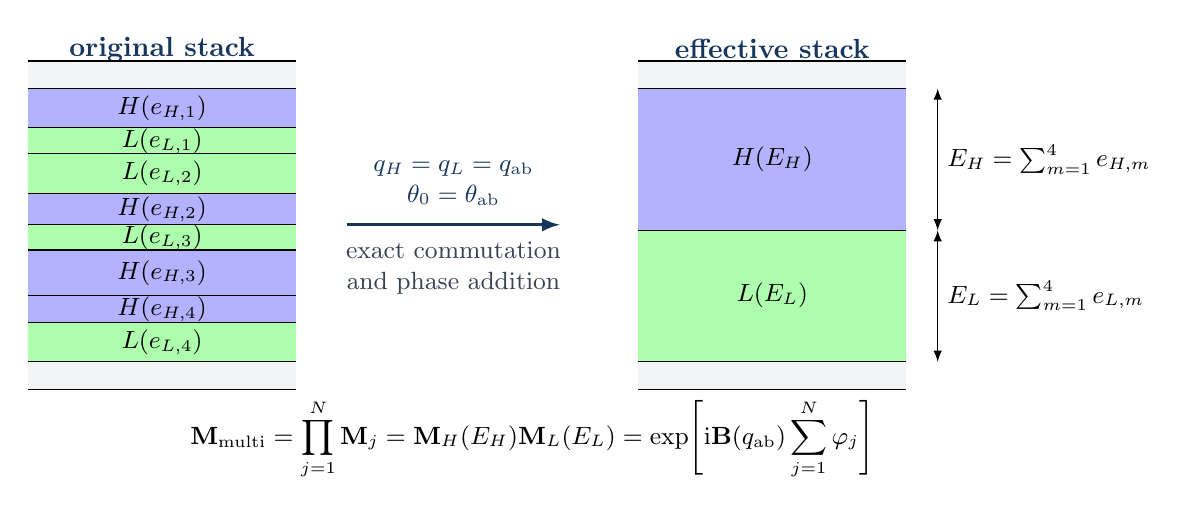
\begin{tikzpicture}[x=1cm,y=1cm,>=latex,font=\small]
  \node[font=\bfseries,navy] at (-4.7,4.05) {original stack};
  \fill[softgray] (-6.4,3.55) rectangle (-3.0,3.90);
  \fill[blue!30]  (-6.4,3.05) rectangle (-3.0,3.55);
  \fill[green!32] (-6.4,2.72) rectangle (-3.0,3.05);
  \fill[green!32] (-6.4,2.22) rectangle (-3.0,2.72);
  \fill[blue!30]  (-6.4,1.82) rectangle (-3.0,2.22);
  \fill[green!32] (-6.4,1.50) rectangle (-3.0,1.82);
  \fill[blue!30]  (-6.4,0.92) rectangle (-3.0,1.50);
  \fill[blue!30]  (-6.4,0.58) rectangle (-3.0,0.92);
  \fill[green!32] (-6.4,0.08) rectangle (-3.0,0.58);
  \fill[softgray] (-6.4,-0.27) rectangle (-3.0,0.08);
  \foreach \y in {-0.27,0.08,0.58,0.92,1.50,1.82,2.22,2.72,3.05,3.55,3.90}
    \draw[thin] (-6.4,\y)--(-3.0,\y);
  \node at (-4.7,3.30) {$H(e_{H,1})$};
  \node at (-4.7,2.88) {$L(e_{L,1})$};
  \node at (-4.7,2.47) {$L(e_{L,2})$};
  \node at (-4.7,2.02) {$H(e_{H,2})$};
  \node at (-4.7,1.66) {$L(e_{L,3})$};
  \node at (-4.7,1.21) {$H(e_{H,3})$};
  \node at (-4.7,0.75) {$H(e_{H,4})$};
  \node at (-4.7,0.33) {$L(e_{L,4})$};

  \draw[very thick,navy,->] (-2.35,1.82)--(0.35,1.82);
  \node[align=center,navy] at (-1.0,2.35)
    {$q_H=q_L=\qab$\\$\theta_0=\theta_{\mathrm{ab}}$};
  \node[align=center,darkgray] at (-1.0,1.27)
    {exact commutation\\and phase addition};

  \node[font=\bfseries,navy] at (3.05,4.05) {effective stack};
  \fill[softgray] (1.35,3.55) rectangle (4.75,3.90);
  \fill[blue!30]  (1.35,1.75) rectangle (4.75,3.55);
  \fill[green!32] (1.35,0.08) rectangle (4.75,1.75);
  \fill[softgray] (1.35,-0.27) rectangle (4.75,0.08);
  \foreach \y in {-0.27,0.08,1.75,3.55,3.90}
    \draw[thin] (1.35,\y)--(4.75,\y);
  \draw[<->] (5.15,1.75)--(5.15,3.55);
  \draw[<->] (5.15,0.08)--(5.15,1.75);
  \node[right] at (5.15,2.65) {$E_H=\sum_{m=1}^{4}e_{H,m}$};
  \node[right] at (5.15,0.92) {$E_L=\sum_{m=1}^{4}e_{L,m}$};
  \node at (3.05,2.65) {$H(E_H)$};
  \node at (3.05,0.92) {$L(E_L)$};

  \node[align=center] at (0, -0.90) {$\displaystyle
  \M_{\rm multi}=\prod_{j=1}^{N}\M_j
  =\M_H(E_H)\M_L(E_L)
  =\exp\!\left[\ii\B(\qab)\sum_{j=1}^{N}\varphi_j\right]$};
\end{tikzpicture}
\caption{Exact compression of a bimaterial stack at the Abelian point. Although the original stack may contain many layers, repetitions, and an arbitrary ordering, its total matrix equals that of two effective layers whose thicknesses are the sums $E_H$ and $E_L$. The equivalence requires a polarization and spectral conditions for which $q_H=q_L$; it does not assert equivalence away from this point.}
\label{fig:compactacion-abeliana}
\end{figure*}

\section{Bimaterial stack}

Consider a stack composed exclusively of $H$ and $L$ layers. At the Abelian angle,
\begin{equation}
q_H=q_L=\qab,
\qquad
\B_H=\B_L=\B(\qab).
\end{equation}
Each layer can be written as
\begin{equation}
\M_j=\exp\!\left(\ii\varphi_j\B(\qab)\right).
\end{equation}
All matrices are functions of the same generator. They therefore commute pairwise, and
\begin{align}
\M_{\mathrm{tot}}
&=\prod_{j=1}^{N}\exp\!\left(\ii\varphi_j\B(\qab)\right)\\
&=\exp\!\left(\ii\B(\qab)\sum_{j=1}^{N}\varphi_j\right).
\label{eq:colapso-total}
\end{align}
Grouping the layers by material gives
\begin{equation}
\sum_j\varphi_j
=\frac{2\pi}{\lambda}\left[
n_H\cos\theta_H\,E_H+n_L\cos\theta_L\,E_L
\right],
\label{eq:fase-acumulada}
\end{equation}
where
\begin{equation}
E_H=\sum_{j\in H}e_j,
\qquad
E_L=\sum_{j\in L}e_j.
\end{equation}

\begin{resultbox}
Identity~\eqref{eq:colapso-total} shows that, in the Abelian limit, the stack no longer retains the layer ordering. Any two sequences with the same accumulated thicknesses $E_H$ and $E_L$ produce the same total matrix under the assumptions of the model. At a fixed wavelength, only the scalar combination in Eq.~\eqref{eq:fase-acumulada} remains. For a full spectrum, it is preferable to retain $E_H$ and $E_L$ separately because their coefficients may depend on $\lambda$.
\end{resultbox}

\section{Validity assumptions}

The derivation requires:
\begin{itemize}
\item planar, homogeneous, isotropic, and nonmagnetic layers;
\item decoupled TE and TM polarizations;
\item the same tangential wave-vector component in every layer;
\item absence of roughness, scattering, and lateral coupling;
\item admittances and phases defined within the $2\times2$ TMM.
\end{itemize}

If $n_H=n_H(\lambda)$ and $n_L=n_L(\lambda)$ are dispersive, then
\begin{equation}
\theta_{\mathrm{ab}}=\theta_{\mathrm{ab}}(\lambda).
\end{equation}
A single angle does not guarantee exact commutation over a broad spectral band unless the dispersions satisfy a special relation. In practice, a band of approximate commutation may be studied through
\begin{equation}
\left\|\comm{\M_H(\lambda)}{\M_L(\lambda)}\right\|
\end{equation}
as a function of $\lambda$ and $\theta_0$.

In absorbing media, the effective indices and angles are complex. The algebraic equation $q_H^2=q_L^2$ remains the formal condition, but a real angle satisfying it may not exist.

The equality $q_H^2=q_L^2$ is the structural condition that nullifies the commutator independently of thickness. It does not exclude accidental commutation at isolated points: for example, if $\sin\varphi_H=0$ or $\sin\varphi_L=0$, one layer matrix may reduce to $\pm\I$ and commute even when the admittances differ. Such degeneracies depend on phase and do not, in general, yield order invariance for arbitrary thicknesses.

\begin{resultbox}
\textbf{Conclusion.} Loss of order memory is not postulated: it follows from all layer matrices becoming exponentials of the same generator. For TM polarization, this coincidence occurs when the reduced admittances of $H$ and $L$ are equal, leading to Eq.~\eqref{eq:resultado-principal}. At this point, the ordered product reduces exactly to a sum of phases, and accumulated variables describe the effective stack space.
\end{resultbox}

\paragraph{Availability.}
The \LaTeX{} source, compiled PDF, and files required to reproduce this preprint are available in
\href{https://github.com/roldannahuelalejadro/thin-film-tmm-order-invariance}{the public GitHub repository}.

\begin{minipage}{\columnwidth}
\section*{References}
\footnotesize
\begin{enumerate}[label={[\arabic*]},leftmargin=2em,itemsep=0pt,topsep=1pt]
\item D. J. Griffiths, \emph{Introduction to Electrodynamics}, 4th ed., Pearson, 2013.
\item P. Yeh, \emph{Optical Waves in Layered Media}, Wiley, 1988.
\item H. A. Macleod, \emph{Thin-Film Optical Filters}, 4th ed., CRC Press, 2010.
\end{enumerate}
\end{minipage}

\end{document}
